\chapter{Introduction}

Predicting the behaviour of complex systems has always been an important goal of scientific research. From predicting the motion of stars and planets in our solar system, to understanding the behaviour of systems showing chaotic behaviours. In history, before scientists were able to find analytical solutions to many problems, they often relied on simulations. A
celebrated example are the astronomical clocks that
were built in Asia and Europe in the period between 1000 and
1500, such as the famous astronomical clock in Prague (1410) or the Zytglogge in Bern (1530). They were used to predict the position of the planets and the constellations, the phases of the moon and its eclipses \cite{bloch2012}.
With the advent of quantum mechanics, a new kind of problems for which no analytical solution is possible was found. Given the high dimensionality of the Hilbert space of quantum many-body systems, classical computers cannot be used to find numerical solutions to this kind of problems. For example, simulating a system of $N=36$ qubit using two double-precision floating-point numbers to store a complex number, would require approximately $2^{N+1} \cross 8$ byte $=$ 1 Terabyte of memory. For every additional qubit, this number would double.
Richard Feynman was the first to propose to use a quantum system to handle this complexity, making use of the law of quantum mechanics itself. In 1982, he proposed to make use of \enquote{one controllable quantum system [to] simulate another} \cite{feynman1982}. In this way, a system of $N$ quantum particles with two states could be simulated using another system of $N$ qubits. The problem is then shifted to finding a system that can be easily tuned and controlled, such that it can be used to simulate a wide range of problems.

\section{Analog and digital quantum simulation}

To tackle this kind of problems, two different approaches have arisen in the past years: (digital) quantum computation and (analog) quantum simulation. In the first case, the information is encoded in qubits that can be found in two computational states $\ket{0}$ and $\ket{1}$. In the latter, a direct mapping between the original problem (i.e. its Hamiltonian) and the simulating system is realized. Among the most promising platforms for quantum computation, we cite the use of superconducting circuits \cite{blais2021a}, Rydberg atoms \cite{wu2021a} and trapped ions \cite{bruzewicz2019}. Whereas for quantum simulation, the use of ultracold quantum gases has gained increasing popularity \cite{bloch2012}.

For example, one of the first system to be simulated with this platform was a system of electrons moving in an ionic periodic lattice potential.  The electrons can be simulated using a gas of fermionic atoms trapped in an optical lattice potential. Here, the periodic potential
through which the particles move is generated externally by making
use of the interference pattern of overlapping laser beams \cite{bloch2008}. It is performing an experiment of this kind that Bloch oscillations, predicted in 1929 by Felix Bloch \cite{bloch1929a}, were directly observed in 1996 in a cloud of ultracold Caesium atoms \cite{dahan1996}, after being observed in 1992 through the emission of THz radiation by the electrons only in a semiconductor super lattice \cite{feldmann1992}. In this case, ultracold gases allowed the first direct observation of a phenomenon that was experimentally inaccessible for a solid state system, proving the potential of this technology. In the following years, new interesting experiments were proposed to simulate the behaviour of different quantum systems. Among them, we cite the use of optical lattices to investigate insulating and superfluid quantum phases \cite{greiner2002}, the use of cavities to mediate long range interactions \cite{landig2016} and the observation of quantized conductance in neutral matter \cite{krinner2015}. In this report, we will focus on the latter, since the project was closely related to it.

\section{Transport experiments}
\begin{figure}
    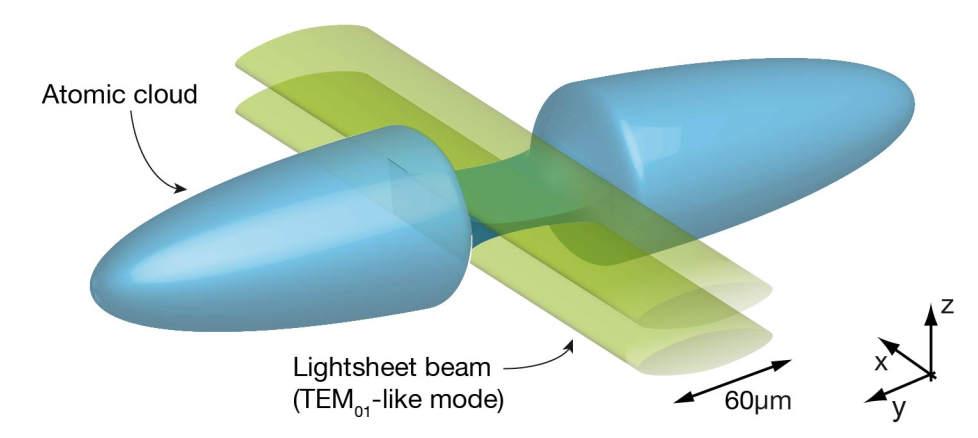
\includegraphics[width=\textwidth]{chapters/chapter_1/figures/reservoir.png}
    \caption{Experimental setup. A cloud of atoms is trapped in a cigar-shaped potential. A blue-detuned $\text{TEM}_{01}$ laser mode propagating in the $x$ direction defined a quasi-2D channel connecting two smoothly connected reservoirs. Figure from Krinner \cite{krinner2015b}.}
    \label{fig:lithium_apparatus}
\end{figure}

Transport experiments study the transport properties of particles moving from one reservoir to another. With an experiment of this kind, Krinner \emph{et al.} were able to observe  quantized conductance in the transport of neutral atoms driven by a chemical potential bias \cite{krinner2015}. Their experiment let them investigate
quantum conductors (systems for which conductance is quantized) with wide control over the channel
geometry and the reservoir properties, such as interaction strength, size and thermalization rate. The basic setup of the experiment is shown in \cref{fig:lithium_apparatus}. A cloud of atoms is radially trapped with a dipole trap realized with a red-detuned laser. Along the $y$ axis the confinement is produced by the magnetic field curvature of the Feshbach coils. This defines a cigar-shaped cloud elongated in the $y$ direction. The cloud is then split in two reservoirs connected by a quasi-2D channel (e.g. due to a blue-detuned $\text{TEM}_{01}$ laser mode in the $x$ direction). The blue-detuned laser creates a repulsive potential that confines the atoms in a quasi-2D region. The experiment is then carried on by creating a chemical potential imbalance between the two reservoirs and studying the conduction of atoms between them. Instead of acting on the chemical potential, different experiments can be realized by creating a temperature or a spin imbalance between the reservoirs.

The focus of this thesis is on the blue-detuned laser generating the 2D channel. In the current experiment, the laser is in a $\text{TEM}_{01}$ mode. The beam is shaped through a series of optical components shown in \cref{fig:beam_shaper}. It is clear that the potential inside the channel region is not uniform along the $y$ direction. The conductance is influenced by this varying potential, and it would be desirable to have a uniform region connecting the two reservoir. The opportunity to create such a uniform 2D channel was previously investigated by Moritz Schmidt in his semester project \cite{schmidt2021}. Schmidt considered two options for generating a uniform light sheet: the use of liquid-crystal spatial light modulators and of custom-made $0-\pi$, top-hat phase-plates. It was found that this second option is more suitable to the experiment, being at the same time  able to satisfy the experimental requirements and considerably cheaper.

\begin{figure}
    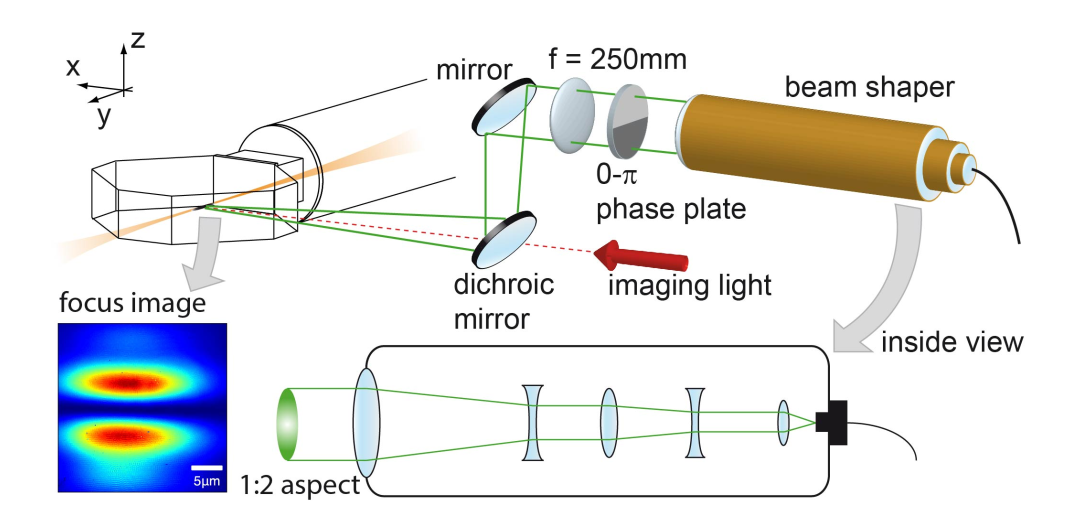
\includegraphics[width=\textwidth]{chapters/chapter_1/figures/beam_shaper.png}
    \caption[short]{Generation of the $\text{TEM}_{01}$ mode for the creation of 2D channel. A set of spherical and cylindrical lenses is used to expand the beam in the $z$ direction. The beam is then sent to a $0-\pi$ phase plate and focused through a \SI{250}{mm} lens on the atomic cloud. Figure from Krinner \cite{krinner2015b}.}
    \label{fig:beam_shaper}
\end{figure}

\section{Outline}
In this report, we analyse and characterize the custom-made phase plate ordered for the creation of the uniform light sheet. The phase plate had already been ordered based on Schmidt's work, but it still had to be tested. In fact, despite knowing its expected behaviour, it was important to check the result that it produced in reality, finding the optimal configuration to make it work.
In the next chapter, we will start reviewing the theory behind atom-light interaction and spatial light modulation. We will offer a brief overview on how atoms interact with light, and how this interaction can be exploited to generate an optical potential. Then, we will discuss how light can be shaped to generate an arbitrary intensity distribution, and therefore an arbitrary potential. To do so, we will review the basics of Fourier optics and the theory behind how phase plates work. Then, we will present the characterization of the phase plate that we received. We will discuss the experimental setup and the methods used to characterize it, especially focusing on the quantities we defined to quantify the \enquote{goodness} of our results. Finally, we will discuss the results highlighting the most important aspects of using the phase plate optimally.